\documentclass{standalone}
\usepackage{tikz}
\usetikzlibrary{patterns, positioning}
\usepackage[sfdefault]{ClearSans} %% option 'sfdefault' activates Clear Sans as the default text font
\usepackage[T1]{fontenc}

\begin{document}
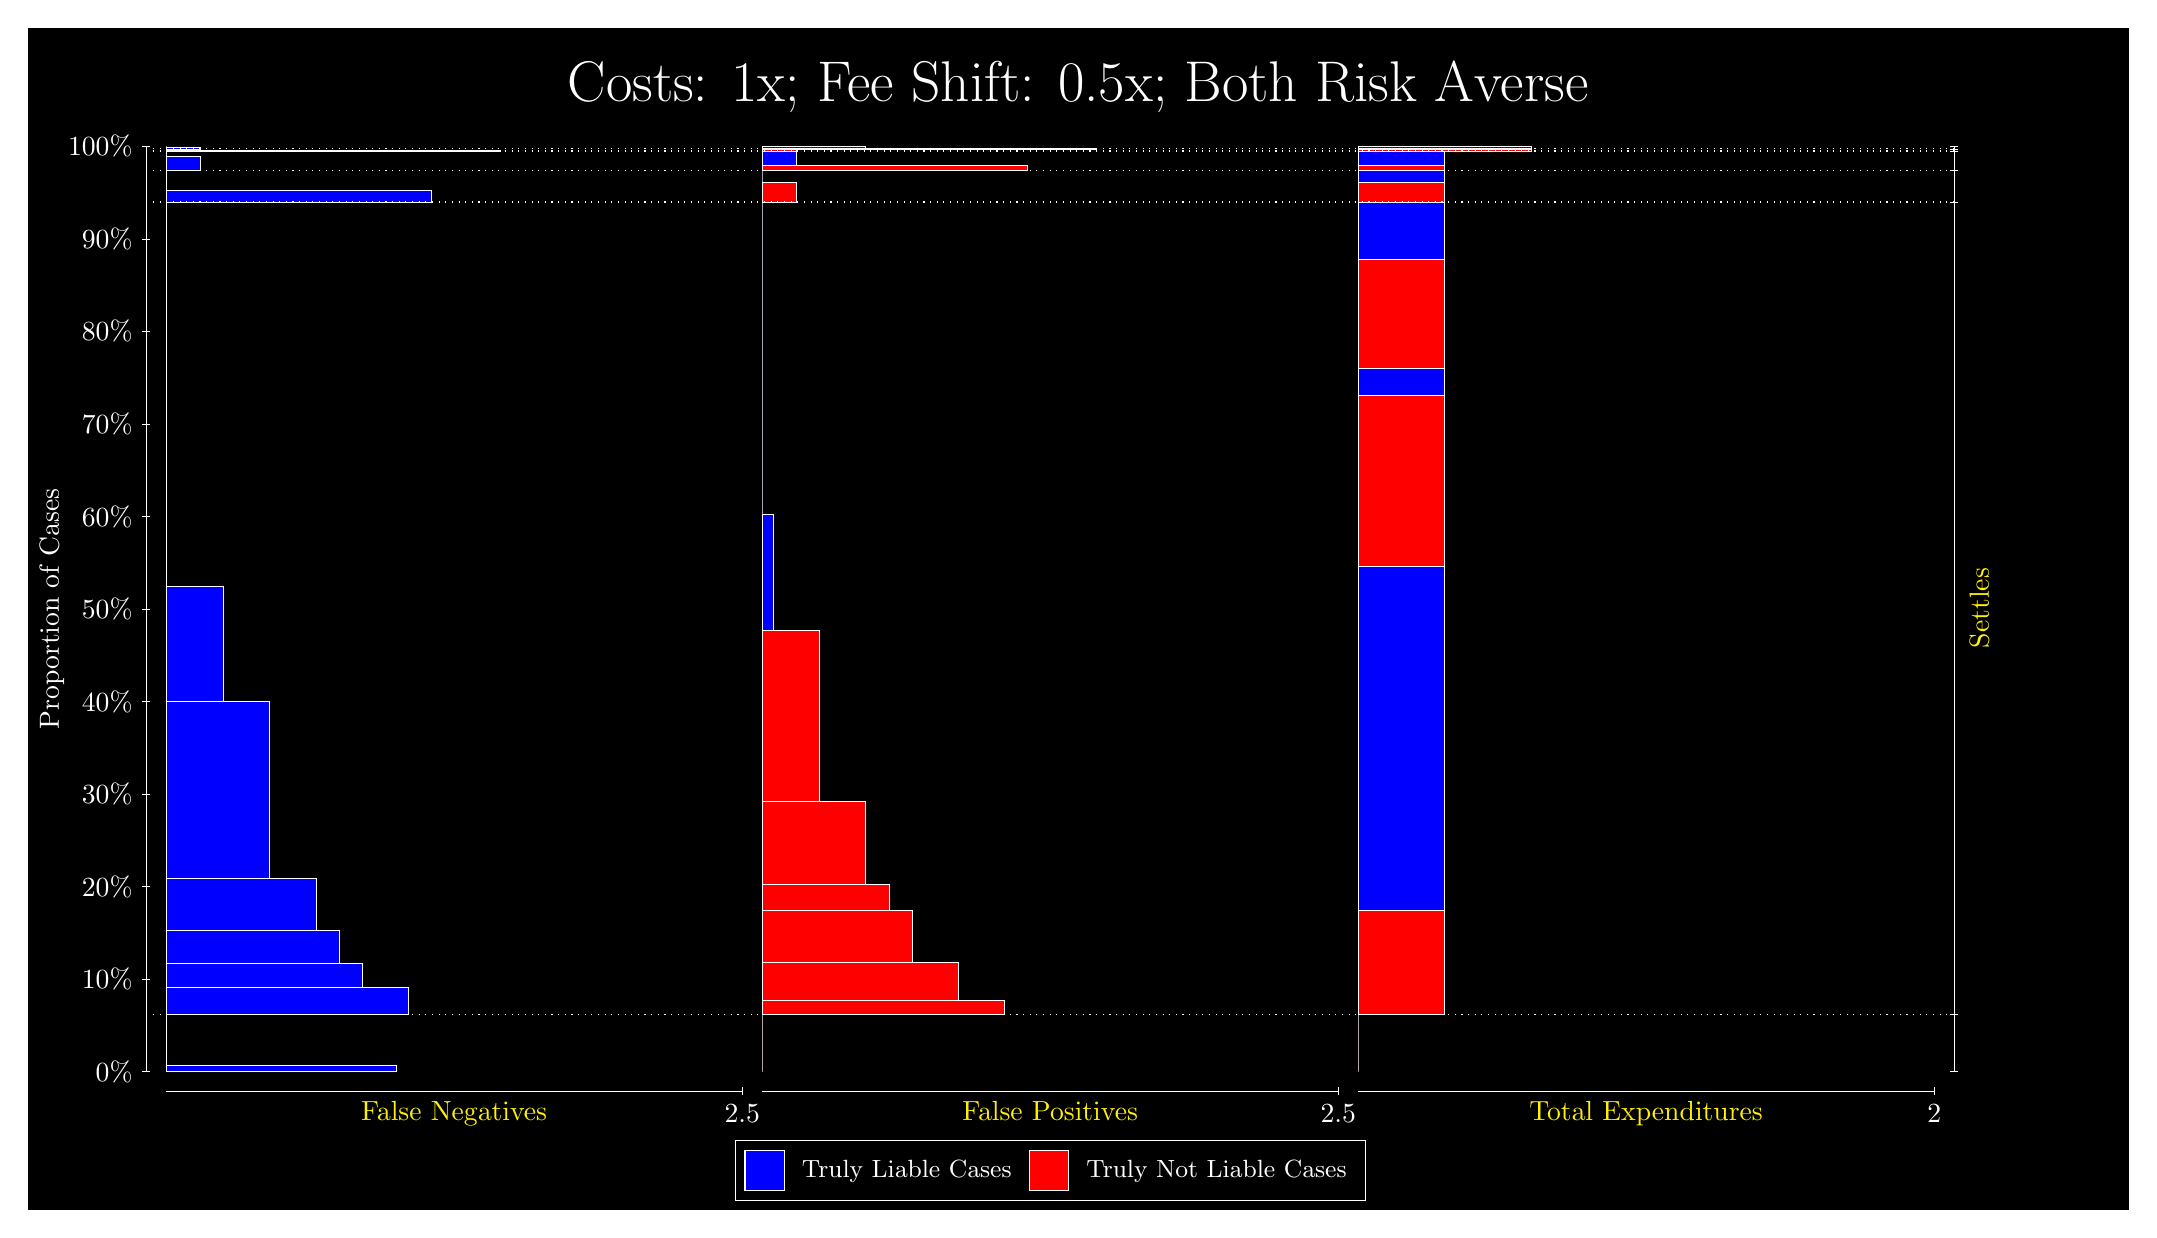
\begin{tikzpicture}
\draw[fill=black] (0,0) rectangle (26.667,15);
\draw[text=white] (0,13.5) rectangle (26.667,15) node[midway] {\huge Costs: 1x; Fee Shift: 0.5x; Both Risk Averse};
\draw[white, very thin] (1.5,1.75) -- (1.5,13.5);
\node[rotate=90, text=white, anchor=center] at (0.3, 7.625) {Proportion of Cases};
\draw[white, very thin] (1.45,1.75) -- (1.55,1.75);
\node[text=white, anchor=east] at (1.45, 1.75) {0\%};
\draw[white, very thin] (1.45,2.925) -- (1.55,2.925);
\node[text=white, anchor=east] at (1.45, 2.925) {10\%};
\draw[white, very thin] (1.45,4.1) -- (1.55,4.1);
\node[text=white, anchor=east] at (1.45, 4.1) {20\%};
\draw[white, very thin] (1.45,5.275) -- (1.55,5.275);
\node[text=white, anchor=east] at (1.45, 5.275) {30\%};
\draw[white, very thin] (1.45,6.45) -- (1.55,6.45);
\node[text=white, anchor=east] at (1.45, 6.45) {40\%};
\draw[white, very thin] (1.45,7.625) -- (1.55,7.625);
\node[text=white, anchor=east] at (1.45, 7.625) {50\%};
\draw[white, very thin] (1.45,8.8) -- (1.55,8.8);
\node[text=white, anchor=east] at (1.45, 8.8) {60\%};
\draw[white, very thin] (1.45,9.975) -- (1.55,9.975);
\node[text=white, anchor=east] at (1.45, 9.975) {70\%};
\draw[white, very thin] (1.45,11.15) -- (1.55,11.15);
\node[text=white, anchor=east] at (1.45, 11.15) {80\%};
\draw[white, very thin] (1.45,12.325) -- (1.55,12.325);
\node[text=white, anchor=east] at (1.45, 12.325) {90\%};
\draw[white, very thin] (1.45,13.5) -- (1.55,13.5);
\node[text=white, anchor=east] at (1.45, 13.5) {100\%};

\draw[white, very thin] (24.457,1.75) -- (24.457,13.5);
\draw[white, very thin] (24.407,1.75) -- (24.507,1.75);
\node[anchor=west] at (24.407, 1.75) {};
\draw[white, very thin] (24.407,2.4788) -- (24.507,2.4788);
\node[anchor=west] at (24.407, 2.4788) {};
\draw[white, very thin] (24.407,12.793) -- (24.507,12.793);
\node[anchor=west] at (24.407, 12.793) {};
\draw[white, very thin] (24.407,13.198) -- (24.507,13.198);
\node[anchor=west] at (24.407, 13.198) {};
\draw[white, very thin] (24.407,13.441) -- (24.507,13.441);
\node[anchor=west] at (24.407, 13.441) {};
\draw[white, very thin] (24.407,13.467) -- (24.507,13.467);
\node[anchor=west] at (24.407, 13.467) {};
\draw[white, very thin] (24.407,13.5) -- (24.507,13.5);
\node[anchor=west] at (24.407, 13.5) {};

\draw[white, very thin, fill=blue] (1.75,1.75) rectangle (4.6775,1.8267);
\draw[white, very thin, fill=red] (1.75,1.8267) rectangle (1.75,2.4788);
\draw[white, very thin, fill=blue] (1.75,2.4788) rectangle (4.8239,2.8188);
\draw[white, very thin, fill=blue] (1.75,2.8188) rectangle (4.2384,3.1191);
\draw[white, very thin, fill=blue] (1.75,3.1191) rectangle (3.9457,3.5426);
\draw[white, very thin, fill=blue] (1.75,3.5426) rectangle (3.6529,4.1996);
\draw[white, very thin, fill=blue] (1.75,4.1996) rectangle (3.0674,6.4492);
\draw[white, very thin, fill=blue] (1.75,6.4492) rectangle (2.4819,7.9164);
\draw[white, very thin, fill=red] (1.75,7.9164) rectangle (1.75,12.793);
\draw[white, very thin, fill=blue] (1.75,12.793) rectangle (5.1167,12.945);
\draw[white, very thin, fill=red] (1.75,12.945) rectangle (1.75,13.198);
\draw[white, very thin, fill=blue] (1.75,13.198) rectangle (2.1891,13.374);
\draw[white, very thin, fill=red] (1.75,13.374) rectangle (1.75,13.441);
\draw[white, very thin, fill=blue] (1.75,13.441) rectangle (5.9949,13.451);
\draw[white, very thin, fill=red] (1.75,13.451) rectangle (1.75,13.467);
\draw[white, very thin, fill=blue] (1.75,13.467) rectangle (2.1891,13.49);
\draw[white, very thin, fill=red] (1.75,13.49) rectangle (1.75,13.5);
\draw[white, very thin, fill=red] (9.3189,1.75) rectangle (9.3189,2.4021);
\draw[white, very thin, fill=blue] (9.3189,2.4021) rectangle (9.3189,2.4788);
\draw[white, very thin, fill=red] (9.3189,2.4788) rectangle (12.393,2.6527);
\draw[white, very thin, fill=red] (9.3189,2.6527) rectangle (11.807,3.1402);
\draw[white, very thin, fill=red] (9.3189,3.1402) rectangle (11.222,3.7973);
\draw[white, very thin, fill=red] (9.3189,3.7973) rectangle (10.929,4.1311);
\draw[white, very thin, fill=red] (9.3189,4.1311) rectangle (10.636,5.1847);
\draw[white, very thin, fill=red] (9.3189,5.1847) rectangle (10.051,7.3558);
\draw[white, very thin, fill=blue] (9.3189,7.3558) rectangle (9.4652,8.823);
\draw[white, very thin, fill=blue] (9.3189,8.823) rectangle (9.3189,12.793);
\draw[white, very thin, fill=red] (9.3189,12.793) rectangle (9.758,13.047);
\draw[white, very thin, fill=blue] (9.3189,13.047) rectangle (9.3189,13.198);
\draw[white, very thin, fill=red] (9.3189,13.198) rectangle (12.686,13.264);
\draw[white, very thin, fill=blue] (9.3189,13.264) rectangle (9.758,13.441);
\draw[white, very thin, fill=red] (9.3189,13.441) rectangle (9.758,13.457);
\draw[white, very thin, fill=blue] (9.3189,13.457) rectangle (9.3189,13.467);
\draw[white, very thin, fill=red] (9.3189,13.467) rectangle (13.564,13.477);
\draw[white, very thin, fill=blue] (9.3189,13.477) rectangle (10.636,13.5);
\draw[white, very thin, fill=red] (16.888,1.75) rectangle (16.888,2.4021);
\draw[white, very thin, fill=blue] (16.888,2.4021) rectangle (16.888,2.4788);
\draw[white, very thin, fill=red] (16.888,2.4788) rectangle (17.986,3.7973);
\draw[white, very thin, fill=blue] (16.888,3.7973) rectangle (17.986,8.1711);
\draw[white, very thin, fill=red] (16.888,8.1711) rectangle (17.986,10.342);
\draw[white, very thin, fill=blue] (16.888,10.342) rectangle (17.986,10.682);
\draw[white, very thin, fill=red] (16.888,10.682) rectangle (17.986,12.07);
\draw[white, very thin, fill=blue] (16.888,12.07) rectangle (17.986,12.793);
\draw[white, very thin, fill=red] (16.888,12.793) rectangle (17.986,13.047);
\draw[white, very thin, fill=blue] (16.888,13.047) rectangle (17.986,13.198);
\draw[white, very thin, fill=red] (16.888,13.198) rectangle (17.986,13.264);
\draw[white, very thin, fill=blue] (16.888,13.264) rectangle (17.986,13.441);
\draw[white, very thin, fill=red] (16.888,13.441) rectangle (19.083,13.457);
\draw[white, very thin, fill=blue] (16.888,13.457) rectangle (19.083,13.467);
\draw[white, very thin, fill=red] (16.888,13.467) rectangle (19.083,13.477);
\draw[white, very thin, fill=blue] (16.888,13.477) rectangle (19.083,13.5);
\draw[white, dotted] (1.5,2.4788) -- (24.457,2.4788);
\draw[white, dotted] (1.5,12.793) -- (24.457,12.793);
\draw[white, dotted] (1.5,13.198) -- (24.457,13.198);
\draw[white, dotted] (1.5,13.441) -- (24.457,13.441);
\draw[white, dotted] (1.5,13.467) -- (24.457,13.467);
\draw[white, very thin] (1.75,1.5) -- (9.0689,1.5);
\node[text=yellow, anchor=north] at (5.4094, 1.5) {False Negatives};
\draw[white, very thin] (9.0689,1.45) -- (9.0689,1.55);
\node[text=white, anchor=north] at (9.0689, 1.45) {2.5};

\draw[white, very thin] (9.3189,1.5) -- (16.638,1.5);
\node[text=yellow, anchor=north] at (12.978, 1.5) {False Positives};
\draw[white, very thin] (16.638,1.45) -- (16.638,1.55);
\node[text=white, anchor=north] at (16.638, 1.45) {2.5};

\draw[white, very thin] (16.888,1.5) -- (24.207,1.5);
\node[text=yellow, anchor=north] at (20.547, 1.5) {Total Expenditures};
\draw[white, very thin] (24.207,1.45) -- (24.207,1.55);
\node[text=white, anchor=north] at (24.207, 1.45) {2};


\node[text=yellow, centered, rotate=90] at (24.777, 7.6361) {Settles};





\draw (12.978300999999998,1.5) node[draw=none] (baseCoordinate) {};
\begin{scope}[align=center]
        \matrix[scale=0.5, draw=white, below=0.5cm of baseCoordinate, nodes={draw}, column sep=0.1cm]{
            \node[rectangle, draw, minimum width=0.5cm, minimum height=0.5cm, fill=blue] {}; &
            \node[draw=none, font=\small, text=white] (B) {Truly Liable Cases}; &
            \node[rectangle, draw, minimum width=0.5cm, minimum height=0.5cm, fill=red] {}; &
            \node[draw=none, font=\small, text=white] (B) {Truly Not Liable Cases}; \\
            };
\end{scope}

\end{tikzpicture}
\end{document}